\documentclass{tufte-handout}

%\geometry{showframe}% for debugging purposes -- displays the margins

\usepackage{amsmath}

% Set up the images/graphics package
\usepackage{graphicx}
\setkeys{Gin}{width=\linewidth,totalheight=\textheight,keepaspectratio}
\graphicspath{{graphics/}}

\title{The Pentose Phosphate Pathway}
\author{}
\date{}  % if the \date{} command is left out, the current date will be used

% The following package makes prettier tables.  We're all about the bling!
\usepackage{booktabs}

% The units package provides nice, non-stacked fractions and better spacing
% for units.
\usepackage{units}

% The fancyvrb package lets us customize the formatting of verbatim
% environments.  We use a slightly smaller font.
\usepackage{fancyvrb}
\fvset{fontsize=\normalsize}

% Small sections of multiple columns
\usepackage{multicol}

% Provides paragraphs of dummy text
\usepackage{lipsum}

% These commands are used to pretty-print LaTeX commands
\newcommand{\doccmd}[1]{\texttt{\textbackslash#1}}% command name -- adds backslash automatically
\newcommand{\docopt}[1]{\ensuremath{\langle}\textrm{\textit{#1}}\ensuremath{\rangle}}% optional command argument
\newcommand{\docarg}[1]{\textrm{\textit{#1}}}% (required) command argument
\newenvironment{docspec}{\begin{quote}\noindent}{\end{quote}}% command specification environment
\newcommand{\docenv}[1]{\textsf{#1}}% environment name
\newcommand{\docpkg}[1]{\texttt{#1}}% package name
\newcommand{\doccls}[1]{\texttt{#1}}% document class name
\newcommand{\docclsopt}[1]{\texttt{#1}}% document class option name

\begin{document}

\maketitle% this prints the handout title, author, and date

\begin{abstract}
\noindent Glucose can enter three pathways; glycolysis, glycogenesis or the pentose phosphate pathway\sidenote{sometimes called the pentose phosphate shunt.}.  This handout will describe the role of this pathway in generating NADPH, nucleosides and the role of reducing equivalents in metabolism.   For more details on this pathway, see Chapter 26 in Biochemistry: A Short Course, available on reserve\cite{Berg2015}.
\end{abstract}

\tableofcontents
\pagebreak
\section{Learning Objectives}

\begin{itemize}
\item Understand the role of Glucose-6-Phosphate Dehydrogenase in regulating flow through the pentose phosphate pathway.
\item Evaluate the role of glucose derived products in fatty acid and triglyceride synthesis.
\item Interpret how the combined regulation of glycolysis, glycogenesis and the pentose phosphate pathway can affect the ability to synthesize lipids.
\item Explain how defects in the pentose phosphate pathway can lead to disease.
\item Understand the difference between \textit{in vitro} antioxidant activity and \textit{in vivo} effectiveness of dietary antioxidants.
\item Explain the role of the liver's cytochrome P450 system, and how this affects detoxification of compounds.
\item Analyse how alcohol is metabolized, and how this is different between moderate and heavy drinkers.
\end{itemize}

\section{Key Vocabulary and Concepts}
\begin{itemize}
	\item NADPH (as opposed to NADH)
	\item Glutathione and the Glutathione Antioxidant System
	\item Antioxidants
	\item Pentoses and Nucleotide Biogenesis
	\item Reducing Equivalents
	\item Favism or G6PDH Deficiency
	\item The Cytochrome P450 System
\end{itemize}

\section{The Pentose Phosphate Pathway}

Recall from the previous lectures, that the flow of glucose between glycogen synthesis, glycolysis and the pentose phosphate pathway is dependent on the rate limiting enzymes of each.  The pentose phosphate pathway is a glucose utilizing pathway which runs parallel to glycolysis, taking Glucose-6-Phosphate and converting it into several products, including NADPH, Ribose 5-phosphate\sidenote{which is used to make nucleotides}, and several glycolytic intermediates including Fructose-6-phosphate and Glyceraldehyde-3-phosphate.  The glycolytic intermediates feed back into glycolysis (see the notes on Glycolysis to see how these pathways reintegrate).

\section{Glucose-6-Phosphate Dehydrogenase}

The first enzyme is the rate limiting and irreversible step of the pentose phosphate pathway and is catalyzed by Glucose-6-Phosphate Dehydrogenase (G6PDH).  G6PDH is activated by elevations of its two substrates NADP\textsuperscript{+} and Glucose-6-Phosphate.  Its activitiy is inhibited by high levels of NADPH.  

\subsection{Nucleotide Biosynthesis and the Pentose Phosphate Pathway}
After the removal of one carbon from the six-carbon ring of glucose, the remaining sugar is a pentose, often a ribose.  Through a complex series of equilibrium reactions, these sugars can be inter-converted in order to generate nucleotides and nucleic acids (ribose in the case of RNA, deoxyribose in the case of DNA).  While non-dividing cells can often recycle their ribose sugars, if a cell is rapidly dividing cells (such as blood cells, skin cells or enterocytes) need substantial ribose to duplicate the six billion bases of DNA in a human cell.  Because of these equilibrium reactions, the pentose phosphate pathway can be the source of riboses when needed, NADPH when needed, or a combination of both.  The stoichiometry of the pentose phosphate pathway therefore can vary depending on needs.  In the case that no ATP is needed, only NADPH this might be the stoichiometry:

\begin{equation}\label{eq:ppp-nadph}
6G6P + 12NADP^+ + 7H_2O \rightarrow 12NADPH + 6CO_2 + 12 H^+ + 12Pi
\end{equation}

But if a combination of energy and NADPH is needed, the stoichiometry might be the following, which should generate 6.8 ATP equivalents/glucose molecule\sidenote{how would this compare with glycolysis to Pyruvate?}:

\begin{equation}
3G6P + 6NADP^+ + 7H_2O + 5NAD^+ + 8ADP + 5Pi \rightarrow 5Pyruvate + 3CO_2 + 6NADPH + 5NADH + 8ATP+ 2H_2O + 8H^+
\end{equation}

In reality its always a mixture, depending on the relative demand of riboses, NADPH and energy.  Do not bother trying to memorize these reactions, but if you want more details about this see the relevant chapter in \citep{Berg2013}.


\section{The Importance of NAPDH}

The most important product of this pathway in terms of nutrition is NADPH\sidenote{This looks like NADH, but is not, it has an extra phosphate group and is generally not inter-convertable with NADH.  However, like NADH it generated largely from Niacin, also known as Vitamin B3.}. While the pentose phosphate pathway is the major source, it is not the only way to generate NAPDH, several other mechanisms exist.  The first is catalyzed by Malate Dehydrogenase:

\begin{equation}
Malate + NADP^+ \rightarrow NADPH + CO_2+ Pyruvate
\end{equation}

This pathway removes malate from the TCA cycle to generate NADPH\sidenote{Think about this, is this cataplerotic, or anaplerotic?}.  A third way to generate NADPH is through an isoform of Isocitate Dehydrogenase:

\begin{equation}
Isocitrate + NADP^+ \rightarrow NADPH + CO_2 + \alpha-Ketoglutarate
\end{equation}

Finally, recently a fourth pathway has emerged, wherin the reduction of 10-TMF to folate\sidenote{This is part of one-carbon metabolism, which will not be covered in this course, but will be covered in NUTR631.} can also generate NADPH in some cells.  The details of this, and its potential as chemotherapeutic target due to its importance in rapidly dividing cells  is described in \citet{Fan2014a}.  The relative importance of these three pathways vary based on cell type and metabolic state, but in most cells the pentose phosphate pathway is prominent.

\subsection{The Role of NADPH in Anabolism}
While glycolysis is a catabolic pathway, the pentose phosphate pathway could be considered an anabolic pathway.  This is because anabolic pathways, notably fatty acid and cholesterol biosynthesis requires a large number of NADPH molecules.  To make one molecule of palmitate (a 16 carbon fatty acid) you need \emph{14 NADPH molecules}.  As described in reaction \ref{eq:ppp-nadph}, you would need more than 6 glucose molecules, just to provide the reducing equivalents to make a palmitate (not including all the energy needed for these reactions, which will be described in the lipid synthesis unit).  Therefore in cells that make a lot of fatty acids and sterols, such as adipose, liver, the mammary glands, testes and adrenal glands, a substantial fraction of glucose is utilized to make NADPH.

\begin{marginfigure}
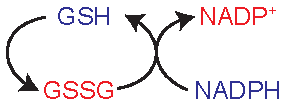
\includegraphics{figures/gsh-nadph.pdf}
\caption{The glutathione:NADPH antioxidant system.  The oxidized form of each molecule is shown in orange, the reduced form is in blue.}
\label{fig:gsh-system}
\end{marginfigure}

\subsection{NADPH is Important for Fighting Oxidative Damage}

The other main role of NADPH is to generate reduced glutathione (GSH) from oxidized glutathione (GSSG) by this reaction, catalysed by Glutathione Reductase:

\begin{equation}
NADPH + GSSG \rightarrow NADP^+ + GSH
\end{equation}

Reduced glutathione is the most important endogenous antioxidant in mammalian cells\sidenote{It also maintains other antioxidants such as Vitamins C and E in their active (reduced) form.}.  When reactive oxygen species, such as free radicals or peroxides are generated, GSH transfers a proton to the oxidative species neutralizing it.  This process is shown in Figure \ref{fig:gsh-system}. Reduced glutathione (GSH) can become oxidized instead of an important protein or lipid in the cell.  The oxidized glutathione (now GSSG) can be regenerated by NADPH, and can continue to scavenge for other potentially dangerous oxidants.  When cells are exposed to oxidative damage, the pentose phosphate pathway is extremely important for mounting the response and restoring equilibrium.

In some cells, such as red blood cells NADPH is the \textit{only} way to reduce glutatione\sidenote{We will talk more about how glutathione is generated in the lecture on non-protein compounds generated from amino acids.}.  This makes red blood cells prone to hemolysis\sidenote{The breakage of red blood cells.} and is a common trait in disorders of the pentose phosphate pathway.

\subsection{Dietary Antioxidants}
While GSH is able to scavenge reactive oxygen species on its own, this system is extended by two key vitamins, C and E.  This occurs via a series of reactions wherein electrons are passed from Vitamins E and/or C to glutathione and then eventually to NADPH.  This is shown in Figure \ref{fig:gsh-system-vitamins}.  Vitamin C is largely soluble, and can scavenge electrons from water soluble areas.  Vitamin E is lipophilic and functions to alleviate the oxidative damage to lipids and lipid-bound proteins.

\begin{figure}
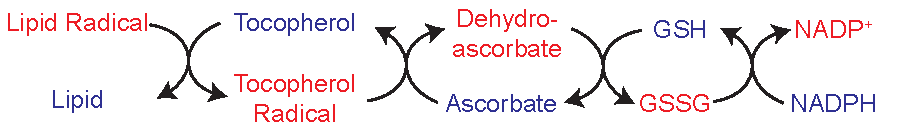
\includegraphics{figures/gsh-nadph-vitamins.pdf}
\caption{The glutathione:NADPH antioxidant system and Vitamins C and E.  The oxidized form of each molecule is shown in orange, the reduced form is in blue.  Ascorbate is the oxidized and active molecular form of Vitamin C, while $\alpha$-tocopherol is the molecular form of Vitamin E}
\label{fig:gsh-system-vitamins}
\end{figure}

Many foods have high levels of antioxidants, and some of these such as the polyphenols present in blueberries have been suggested to alleviate oxidative damage, and reduce some chronic diseases \citep{Pandey2009}.  While it is true that these compounds have some \textit{in vitro} anti-oxidant activity in isolation, there is very little evidence that these anti-oxidants have relevant functional antioxidant ability in humans.  This is thought to be due to poor bioavailability, potency and cellular levels relative to Vitamins C and E.  While Vitamins C and E are both necessary for humans at low quantities, the benefits of extra supplementation are less clear.  A recent systematic review of antioxidant supplementation (including Vitamins A,C,E and Selenium\sidenote{An essential cofactor for Glutathione peroxidase, an enzyme which removes peroxide using reduced glutathione.}) not only demonstrated no beneficial effects on mortality, but found that supplementation led to a 4\% increase in mortality \citep{Bjelakovic2012}.  It is possible that there may be some benefits in populations exposed to substantial oxidative stress (people who smoke, live in areas with high levels of air pollution, consume large amounts of alcohol or individuals with non-alcoholic fatty liver disease), but in the general population there seems to be no measurable benefit of supplementation.  

\subsection{NADPH is Required for Innate Immunity}

A third major role of NADPH is the oxidative burst.  One way in which immune cells can try to destroy invading cells is to use NADPH  to generate reactive oxygen species.  Phagocytic cells first engulf the bacteria or fungi, then using the enzyme NADPH Oxidase, use NADPH to generate a superoxide molecule.  This reacts with proteins, membranes and nucleic acids in the bacteria eventually destroying the invading cell.  As you might expect this destructive process must be tightly controlled to avoid oxidative damage to normal tissues.

\subsection{Disorders of the Pentose Phosphate Pathway}

\newthought{Mutations in G6PDH}
Mutations in the gene for G6PDH (symbol is \textit{G6PD}) can have varying effects depending on the particular amino acid that is changed\sidenote{\textit{G6PD} is on the X-chromosome, so primarily this defect affects males.}.  In the most serious cases, where there is effectively no detectable G6PDH activity.  This is the most common enzymatic defect, affecting an estimated 400 million people worldwide.  These patients are extremely prone to oxidative damage, and can have a buildup of Glucose-6-Phosphate.  They are also very sensitive to certain infections and foods, notably fava beans\sidenote{This disorder was once known as \emph{Favism}, and has been described since antiquity.  For more details see the review by \citet{Luzzatto2018}.}  Interestingly, carriers of the mutant G6PD allele also have partial immunity to malaria, which requires host-derived NADPH\sidenote{Here is a public health issue to consider (or write a report on if you are really interested).  One of the major antimalarials is a drug called primaquine.  This drug is effective at reducing NAPDH levels and reducing susceptibility to malaria.  However, if that person has a deficiency in \textit{G6PD}, they will be probe to primaquine-induced hemolysis, because this can exacerbate inborn defects in NADPH production \citep{Chatterjea1961}.  Since both malaria, and \textit{G6PD} deficiency are both most prevalent in sub-Saharan Africa, it is important that individuals be screened prior to primaquine administration \citep{Howes2013}.}.  This selective benefit may explain why, in contrast to other inborn errors of metabolism, Favism has persisted in human populations.

\section{Alcohol Metabolism}

Almost three quarters of the population of the United States report drinking alcohol in the past year with a wide range of consumption across the population\sidenote{This is \emph{not} a normal distribution, as the top decile of alcohol consumers average over 10 drinks per day.  See the visualization at \url{https://www.washingtonpost.com/news/wonk/wp/2014/09/25/think-you-drink-a-lot-this-chart-will-tell-you} to see this skewed distribution.}.  Virtually all the alcohol we ingest is absorbed, and the vast majority of it must be metabolized by the liver.  There are two major pathways that are engaged in this process.  The first involves this sequence, catalyzed by alcohol dehydrogenase (ADH),  aldehyde dehydrogenase (ALDH) and Acetyl-CoA Synthase (ACS).  This is diagrammed in Figure \ref{fig:alcohol-adh}A:


\begin{figure}
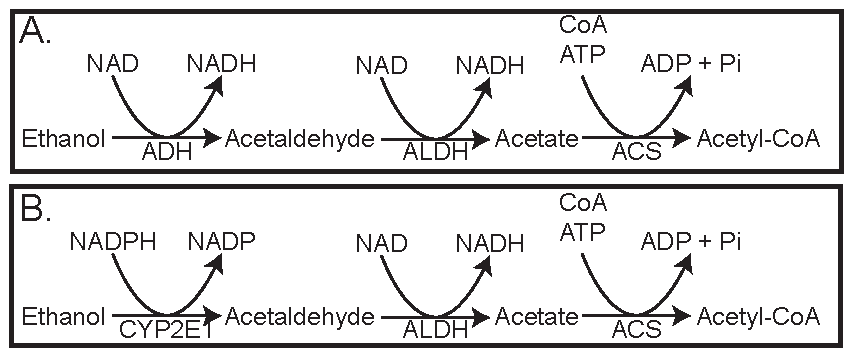
\includegraphics{figures/alcohol-adh.pdf}
\caption{Alcohol metabolism into Acetyl-CoA via A) Alcohol Dehydrogenase or B) \textit{CYP2E1}.}
\label{fig:alcohol-adh}
\end{figure}

Hopefully by now you can determine that for the ADH-dependent pathway there are 15 ATP equivalents generated, and one ATP used, so the net result is 14 ATP per ethanol molecule.  If you recall from the energy balance lecture, the Atwater value of ethanol is 7 kcal/g so more than carbohydrates or protein, but a bit less than lipids.  Still, that is a lot of energy to deliver to the liver.  The result is that the Acetyl-CoA is often diverted to lipogenesis, which can contribute to NAFLD, and while cataplerosis may be activated (recall that Acetyl-CoA activates Pyruvate Carboxylase, there is no corresponding increase in amino acids or glycerol from other tissues.  This results in depletion of glycogen from the liver and the reduction of TCA intermediates).  The situation gets worse in chronic drinkers, where the ADH enzyme cannot process the alcohol effectively enough.  This results in the transcriptional activation of Cytochrome P450 enzyme E1 (CYP2E1).  This set of reactions (shown in Figure \ref{fig:alcohol-adh}B) now \emph{use} NADPH rather than generating NADH.  This means that the liver's antioxidant capacity is reduced, and the chances of oxidative stress and chronic liver damage (known as alcoholic fatty liver disease) can occur.  While NAFLD is increasing in prevalence, most end-stage liver disease is due to chronic alcohol consumption.  This is thought to be a combination of lipid accumulation and oxidative damage.

\newthought{The Cytochrome P450 system detoxifies many other substances.}  In addition to alcohol, other Cytochrome P450 enzymes cause the enzymatic alteration (generally for purposes of stabilization and excretion) of many other compounds.  This is an important process whereby the liver prepares and removes inessential compounds from our bodies.  An interesting example is caffeine, which is hydroxylated by \textit{CYP2E2}.  There are common variants in \textit{CYP1A2} that result in slower metabolism of caffeine.  These individuals have higher sustained spikes in caffeine in their blood, and may be at slightly higher risk for caffeine-induced hypertension.

\newthought{Genetic variation in \textit{ALDH2} is the most common metabolic enzyme variant worldwide.}  Approximately 30-40\% of individuals of Asian descent have only one active copy of \textit{ALDH2} the second enzyme in both the alcohol metabolism pathways we have described.  This results in elevations in both ethanol and acetaldehyde for longer periods of time, often resulting in flushing, nausea, heart palpitations and worsened hangovers.  This differential metabolism is also associated with increased risks of liver disease and alcohol-associated cancers at equivalent alcohol intakes.

\bibliography{library}
\bibliographystyle{plainnat}

\end{document}
